\section{Multiple Shooting}
\begin{mini*}|s|
{w}{\sum_{k=1}^NI_k^2 -W_u u_{k-1}^2}
{}{}
\addConstraint{f(x_0, u_0) - x_1 = 0}
\addConstraint{f(x_k, u_k) - x_{k+1} = 0}
\addConstraint{\vdots}
\addConstraint{f(x_{N-1}, u_{N-1}) - x_{N} = 0}
\addConstraint{u_{max} \geq u_k \geq u_{min}}{}
\end{mini*}
Where $f(.)$ is the trajectory from $x_k$ to $x_{k+1}$. The problem can be formulated in CasADI by modifying algorithm \ref{alg:SingleShooting_Integraion} to capture intermediate states, bounds and constraints:



The RK4-integrator can be replaced by collocation constraints resulting in a direct collocation scheme.

\subsection{Interfacing IPOPT in CasADI}

\subsubsection{Implementation}
\begin{algorithm}[H]
\SetAlgoLined
\KwData{$x = MX \in \mathbb{R}^{N+1}, u = \in \mathbb{R}^{N}, h, N, M$}
define f as chosen integrator

add initial condition bounds
 \For{$i$ = 0 : $N-1$}{
    $x_{int}, Q_k = f(@SIR,@Cost, x_k, u_k, h)$\\
    $J += Q_k$\\
    add $u_{min} - u_k, u_k - u_{max}$ to bounds\\
    add $x_{min}-x_k, x_k - x_{max}$ to bounds\\
    add $x_{int} - x_{k+1}$ to constraints\\
    set $u_{k,0}$\\
    set $x_{k, 0}$
 }
 \KwRet{$x_k, J,X_0,U_0$, bounds, constraints}
 \caption{Multiple-Shooting problem construction and integration (RK4)}
 \label{alg:MultipleShooting_Integraion}
\end{algorithm}

In order to get comparable performance to single shooting, the multiple shooting scheme should be initialized with the same initial trajectory for the lifted states. RK4 and 
\subsubsection{Results}
Simulating with parameters defined in section \ref{ch:Problem_Parameters} yields trajectories, bounds multipliers, constraints multipliers and objective values respectively shown in figure \ref{fig:MS_Traj_SD_IPOPT}, \ref{fig:MS_Bounds_SD_IPOPT}, \ref{fig:MS_Cons_Obj_IPOPT} (Using the same initial trajectory as in single shooting). In order to illustrate the advantages of lifting the states, another simulation can be run using $x_0$ as initial value for all lifted states.

\begin{figure}[H]
    \centering
    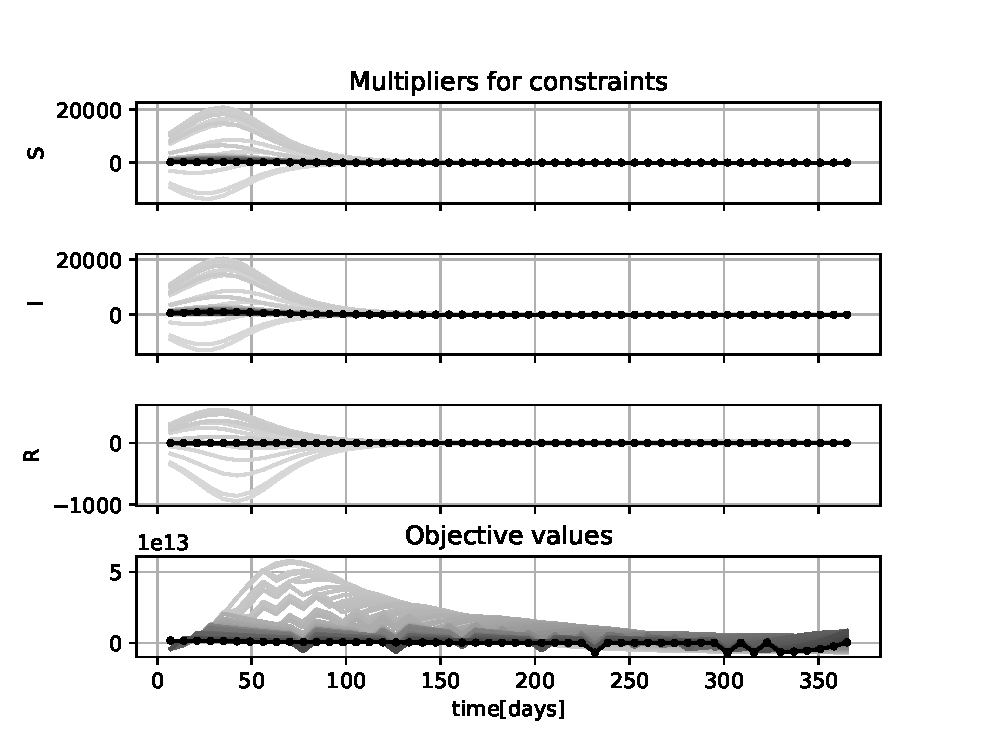
\includegraphics[width=.8\textwidth]{pythonProject/Figures/Multiple_Shooting_obj_con_IPOPT_traj_initial_Social_Distancing.eps}
    \caption{Trajectories with multiple shooting using IPOPT}
    \label{fig:MS_Traj_SD_IPOPT}
\end{figure}

\begin{figure}[H]
    \centering
    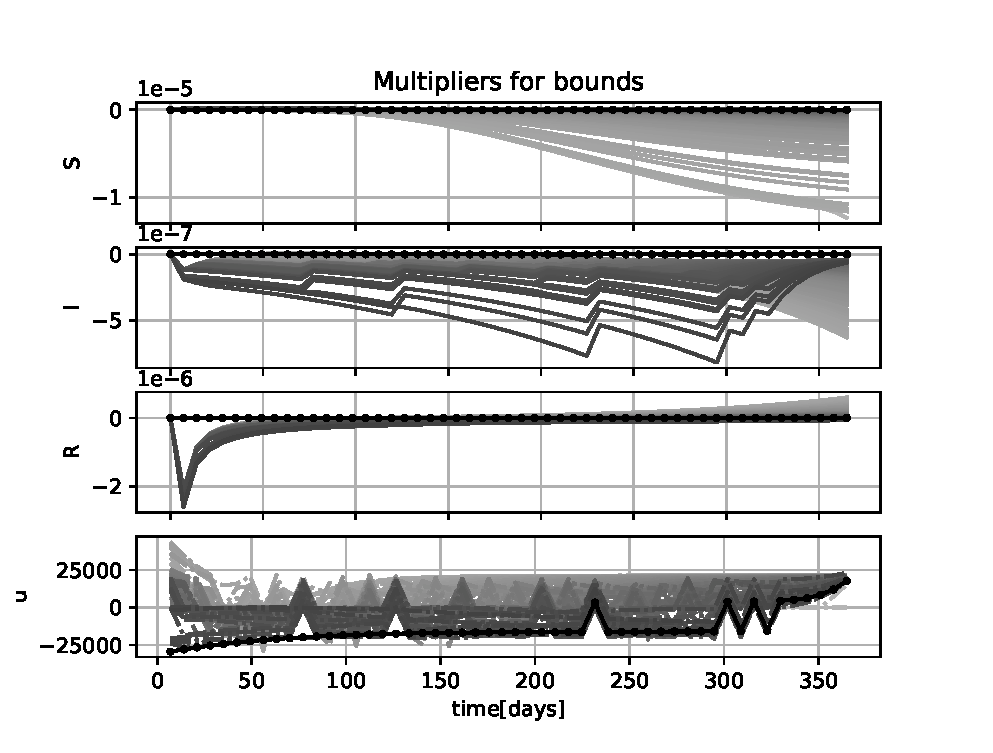
\includegraphics[width=.8\textwidth]{pythonProject/Figures/Multiple_Shooting_bounds_IPOPT_traj_initial_Social_Distancing.eps}
    \caption{Boundary multipliers with multiple shooting using IPOPT}
    \label{fig:MS_Bounds_SD_IPOPT}
\end{figure}


\begin{figure}[H]
    \centering
    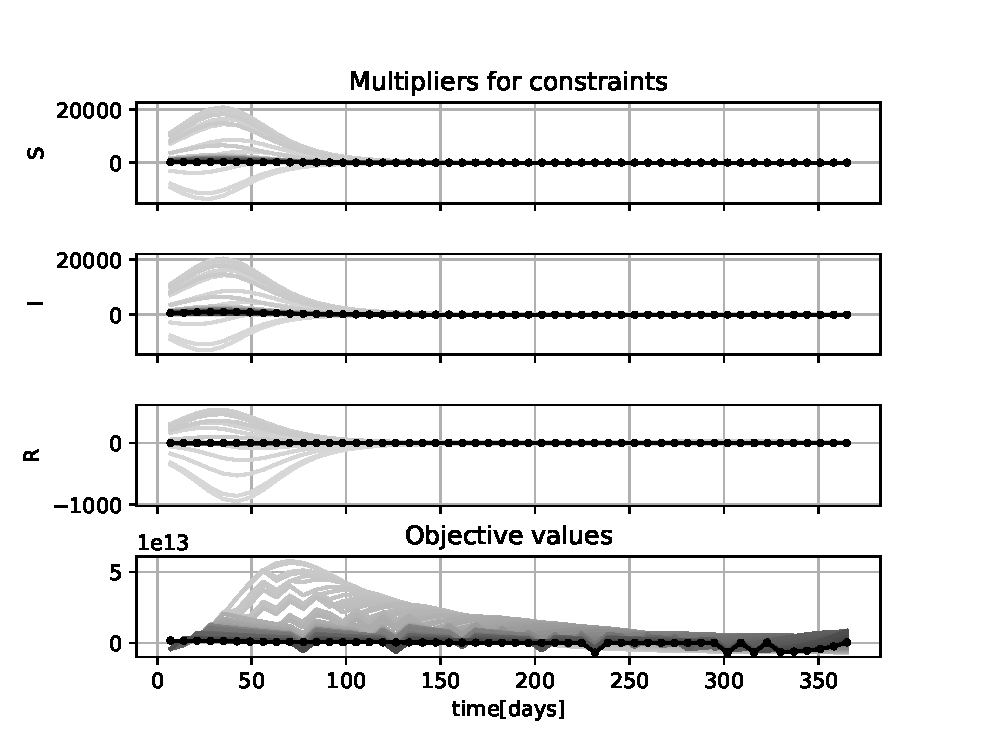
\includegraphics[width=.8\textwidth]{pythonProject/Figures/Multiple_Shooting_obj_con_IPOPT_traj_initial_Social_Distancing.eps}
    \caption{Constraints and objective values multiple shooting using IPOPT}
    \label{fig:MS_Cons_Obj_IPOPT}
\end{figure}

Solving the problem with $x_0$ as initial value for all lifted states yields trajectory shown in figure \ref{fig:MS_Traj_IPOPT}.

\begin{figure}[H]
    \centering
    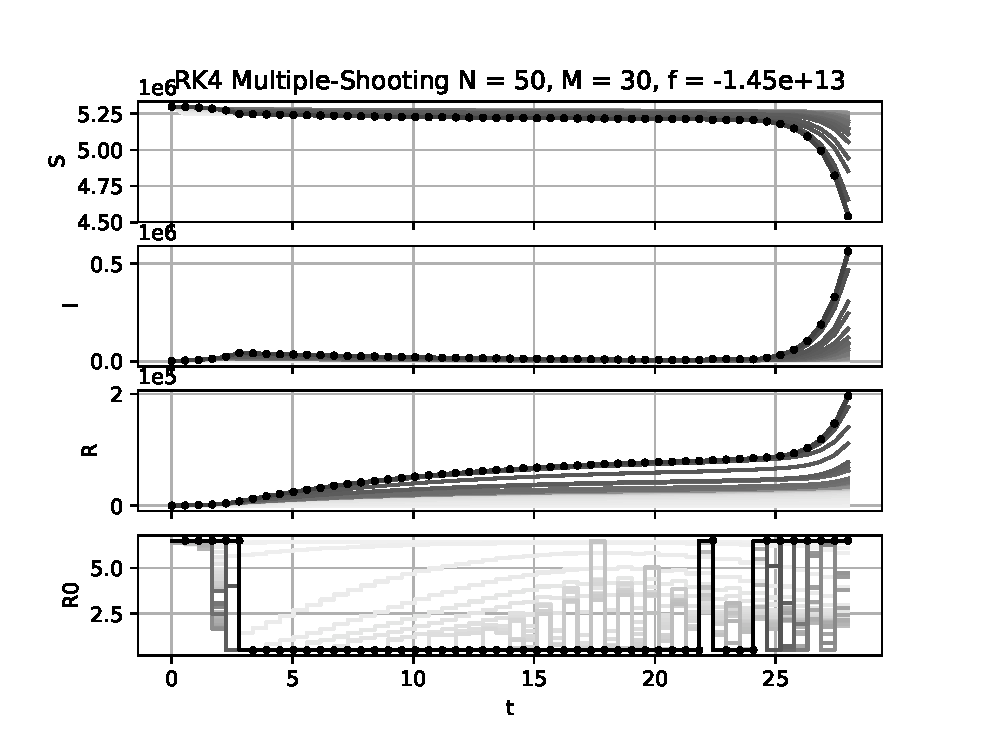
\includegraphics[width=.8\textwidth]{pythonProject/Figures/Multiple_Shooting_Trajectory_IPOPT.eps}
    \caption{Trajectories with multiple shooting using IPOPT}
    \label{fig:MS_Traj_IPOPT}
\end{figure}

\subsubsection{Discussion}
The lifted states enables the problem to be solved to a better objective value at the cost of more iterations. The partially concave objective function makes the solver converge towards the same local solution as in single shooting, but postpones the lockdown phase for another day.

Choosing infeasible initial conditions results in a better solution of the problem. By setting all lifted states to $x_0$, the IPOPT-solver converges towards a solution with a much longer lockdown-phase, and is effectively able to avoid an epidemic until the end of the control horizon, where the lockdown policies are lifted. The local solution lifts the lockdown-restrictions for a one-day period before the permanent lifting. This would not have a good effect in reality, but illustrates the need for an objective function rewarding gradual lifting of lockdowns. 


